%__________________________________PREAMBLE_________________________________%
\documentclass[12pt,english]{article}
\usepackage[a4paper, left = 2cm,%
            right=2cm,top=2cm,bottom=2cm,%
            footskip=.25in]{geometry}
\usepackage{amsfonts, amsmath, amssymb, physics}
\usepackage[utf8]{inputenc}
\usepackage[english]{babel}
\usepackage[backend=biber, citestyle=nature]{biblatex}
\usepackage[nottoc]{tocbibind}
\usepackage{indentfirst, halloweenmath, calligra, %
            esint, graphicx, hyperref, xcolor, float}
\hypersetup{
  colorlinks   = true, %Colours links instead of ugly boxes
  urlcolor     = blue, %Colour for external hyperlinks
  linkcolor    = blue, %Colour of internal links
  citecolor   = red %Colour of citations
}
\graphicspath{{./images/}}
%__________________________________COMMANDS_________________________________%
\addbibresource{ref.bib}
%_____________
\setlength{\parindent}{2em}
\setlength{\parskip}{0em}
%_____________
\newcommand{\dmr}[1]{\, \mathrm{d}#1} %command for the straight d after the integral
\newcommand{\intt}[2]{\int_{#1}^{#2}} %easy integral command 
%_____________
\DeclareMathAlphabet{\mathcalligra}{T1}{calligra}{m}{n}
\DeclareFontShape{T1}{calligra}{m}{n}{<->s*[2.3]callig15}{}
\newcommand{\curly}[1]{\ensuremath{\mathcalligra{#1}}}
%_____________
\let\oldhat\hat
\renewcommand{\vec}[1]{\boldsymbol{#1}}
\renewcommand{\hat}[1]{\oldhat{\boldsymbol{#1}}}
\newcommand{\ar}[1]{\overset{\rightharpoonup}{#1}}
%_____________
\newcommand{\comment}[1]{}
%___________________________________________________________________________%
\title{\textbf{Electrodynamics Topic 1}\\ 
\large Green's Function \& Retardation\\ 
\small Lecture 1, 2}
\date{\today}
% \author{Joey Liang}
\begin{document}
%_______________________________Title Page__________________________________%
\pagenumbering{gobble}
\begin{titlepage}
    \maketitle
    \vfill
    \emph{DISCLAIMER: I, Jiongyu Liang, am NOT the original authour of the content presented %
        below, the following is just electronic type-up of the lecture note produced %
        by Dr. Oleg Tretiakov.}
\end{titlepage}
\cleardoublepage
\pagenumbering{arabic}
%__________________________________TOC______________________________________%
\newpage
\tableofcontents
\newpage
%_______________________________DOCUMENT____________________________________%

\newpage
\section{Introduction}
The Green's function is used for solving inhomogeneous linear ordinary partial differential equations(PDE) subject to some initial or/and boundary conditions. In the context of electrodynamics, we use Green's functions to solve Maxwell's Equations for the EM potential $\phi$ and $\vec{A}$.



\section{Green's function method for static Problems}


\subsection{Simple Example}
\begin{figure}[H]
    \centering
    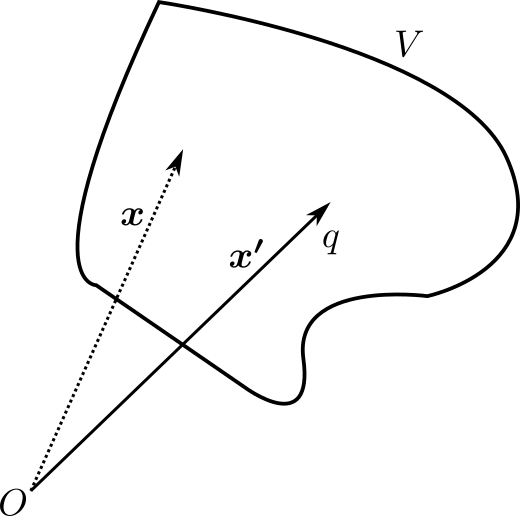
\includegraphics[width = 0.45\textwidth]{chargeinV.png}
    \caption{A volume $V$ contating a charge $q$.}
    \label{fig:chargeinV}
\end{figure}
Consider Gauss' law for a point charge sitting at $\vec{x'}$(Fig.~\ref{fig:chargeinV}). In some volume $V$, we have
\begin{equation*}
    \div \vec{E}(\vec{x'}) = \frac{q}{\varepsilon_0}\delta(\vec{x}-\vec{x'}).
\end{equation*}
Recall that for static charges,
\begin{equation*}
    \vec{E} = -\grad \Phi.
\end{equation*}
Thus, we arrive at the Possion's equation for a static charge
\begin{equation}
    \laplacian\Phi(\vec{x}) = -\frac{q}{\varepsilon_0}\delta(\vec{x} - \vec{x'}).
\end{equation}

Now, imposing the following boundary conditions
\begin{equation}
    \Phi(x) \to \phi_s \text{ as } \abs{\vec{x} - \vec{x'}} \to \infty. \label{eqn:bcFreespace}
\end{equation}
From the following realtionship (Note that $\curly{r} = \vec{x} - \vec{x'}$)
\begin{subequations}
    \begin{align}
        \div\left(\frac{\hat{\curly{r}}}{\curly{r}^2}\right) & = 4\pi\delta(\vec{\curly{r}})           \\
        \grad(\frac{1}{\abs{\curly{r}}})                     & = -\frac{\hat{\curly{r}}}{\curly{r}^2},
    \end{align}
\end{subequations}
we can establish the following
\begin{equation}
    \Phi(x) = q \underbrace{\frac{1}{4\pi\varepsilon_0}\frac{1}{\abs{\curly{r}}}}_{=G_0(\curly{r})} + \phi_s
\end{equation}
Here, $G_0$ is called the \textbf{free-space Green's function}. Free-space implies that $\Phi(\vec{x}) \to 0$ as $\curly{r} \to \infty$. In other words, $G_0$ is the solution of
\begin{equation}
    \laplacian G_0(\curly{r}) = -\frac{1}{\varepsilon_0} \delta(\curly{r}) \label{eqn:Gfn5}
\end{equation}
in the volume $V$, subject to the boundary condition (\ref{eqn:bcFreespace}) with $\phi_s = 0$.

Now, consider a collection of point charges $q_i$ at $\vec{x_i}$ where $\vec{x_i} \in V$ subject to the same boundary condition (\ref{eqn:bcFreespace}). Then by the principle of superposition
\begin{equation}
    \laplacian \Phi_{\text{total}}(\vec{x}) = \sum_{i = 1}^{N}\laplacian\Phi(\vec{x}) = - \sum_{i = 1}^{N} \frac{q_i}{\varepsilon_0} \delta(\curly{r}),
\end{equation}
and the solution is
\begin{subequations}\label{eqn:FreeGreenSol}
    \begin{align}
        \Phi_{\text{total}}(\vec{x}) = \sum_{i = 1}^{N} \Phi_i(\vec{x}) = \sum_{i = 1}^{N} q_i G_0 + \phi_s \\
        \implies \text{Continuum Limit} = \iiint_{V} \rho(\vec{x'}) G_0 + \phi_s \dmr{\vec{V}}.
    \end{align}
\end{subequations}
Thus, Green's function is essentially the linear response of the system at $\vec{x}$ to a point source at $\vec{x}$.


\subsection{The General Case}
The previous example is simple because the boundary conditions are trivial. In order to obtain the general Green's function solution for arbitrary boundary conditions, we need to use the first and second Green's identities.
\begin{subequations}
    \begin{align}
         & \iiint_{V}\left[\Phi\laplacian\Psi + \grad\Phi \cdot \grad\Psi\right] \dmr{\vec{V}} = \oiint_S (\Phi\grad\Psi)\cdot\dmr{\vec{S}} \label{eqn:G1ID}                          \\
         & \iiint_{V}\left[\Phi\laplacian\Psi - \Psi\laplacian\Phi\right] \dmr{\vec{V}} = \oiint_S \left[ \Phi\grad\Psi - \Psi\grad\Phi \right] \cdot \dmr{\vec{S}}; \label{eqn:G2ID}
    \end{align}
\end{subequations}
Where $\Phi$ and $\Psi$ are scalar functions, and the identities follow essentially from the divergence theorem.

Now, let $\Phi$ be the potential and $\Psi(\vec{x}) = G(\vec{x}, \vec{x'})$. Then the second identity (\ref{eqn:G2ID}) becomes
\begin{equation}
    \begin{split}
        \iiint_{V} \Phi(\vec{x'}) \nabla^{'2} G &\dmr{\vec{V}} \\
        &= \iiint_{V} G \nabla^{'2} \Phi(\vec{x'}) \dmr{\vec{V}} + \oiint_S \left[ \Phi(\vec{x'}) \grad' G - G\grad'\Phi(\vec{x'})  \right] \dmr{\vec{S}}. \label{eqn:Green9}
    \end{split}
\end{equation}
Now, using Eqn.~\ref{eqn:Gfn5}, we arrive at
\begin{equation}
    \iiint_{V} \Phi(\vec{x'}) \nabla^{'2} G \dmr{\vec{V}} = -\frac{1}{\varepsilon_0}\iiint_V \Phi(\vec{x'})\delta(\vec{x}-\vec{x'})\dmr{\vec{V}} = -\frac{1}{\varepsilon_0}\Phi(\vec{x}). \label{eqn:Green10}
\end{equation}
And, by Possion's equation $\laplacian\Phi = - \frac{\rho}{\varepsilon_0}$, we have
\begin{equation}
    \iiint_{V} G \nabla^{'2} \Phi(\vec{x'}) \dmr{\vec{V}} = -\frac{1}{\varepsilon_0}\iiint_V G(\vec{x},\vec{x'})\rho(\vec{x'})\dmr{\vec{V}}. \label{eqn:Green11}
\end{equation}
Thus, using Eqn.~\ref{eqn:Green10} \& Eqn.~\ref{eqn:Green11}, Eqn.~\ref{eqn:Green9} becomes
\begin{equation}
    \begin{split}
        \Phi(\vec{x}) = \iiint_V \rho(\vec{x'})G(\vec{x}, \vec{x'}) \dmr{\vec{V}} &- \varepsilon_0 \oiint_S\nabla'G(\vec{x}, \vec{x'})\Phi(\vec{x'})\cdot\dmr{\vec{S}}\\
        &+ \varepsilon_0\oiint_S\nabla'\Phi(\vec{x'})G(\vec{x}, \vec{x'})\cdot\dmr{\vec{S}}. \label{eqn:GenGreenSol}
    \end{split}
\end{equation}
This is known as the solution for the \textbf{general Green's function}.

Comparing general Green's function solution Eqn.~\ref{eqn:GenGreenSol} with the free-space case Eqn.~\ref{eqn:FreeGreenSol}, we see that in both cases the $1^{st}$ term on the RHS corresponding to the ``response" to a distribution of charges. The remaining terms correspond to the boundary conditions. In the case of Eqn.~\ref{eqn:GenGreenSol}, there are two terms associated with boundary conditions.


\subsection{Boundary Conditions}

\subsubsection{Dirichlet Boundary Conditions}
In the case of Dirichlet BC, we specify only $\Phi(\vec{x})$ on the boundary surface $S$. An example being
\begin{equation}
    G(\vec{x_s}, \vec{x'}) = 0,
\end{equation}
where $\vec{x_s} \in S, \; \vec{x'} \in V$. So Eqn.~\ref{eqn:GenGreenSol} becomes
\begin{equation*}
    \Phi(\vec{x}) = \iiint_V \rho(\vec{x'})G(\vec{x}, \vec{x'}) \dmr{\vec{V}} - \varepsilon_0 \oiint_S\nabla'G(\vec{x}, \vec{x'})\Phi(\vec{x'})\cdot\dmr{\vec{S}}.
\end{equation*}
Furthermore, it can be shown using Green's second identity (Eqn.~\ref{eqn:G2ID}), that the Dirichlet Green's function satisfies the reciprocity theorem
\begin{equation}
    G(\vec{x'}, \vec{x}) = G(\vec{x}, \vec{x'}).
\end{equation}

Thus, once we have specified $\Phi(\vec{x})$ on $S$, we have an unique solution:
\begin{equation}
    \Phi(\vec{x} \in V) = \iiint_V \rho(\vec{x'})G(\vec{x}, \vec{x'}) \dmr{\vec{V}} - \varepsilon_0 \oiint_S\nabla'G(\vec{x}, \vec{x'})\Phi(\vec{x'})\cdot\dmr{\vec{S}}.
\end{equation}
The free-space Green's function (Eqn.~\ref{eqn:FreeGreenSol}) is an example of of a Dirichlet Green's function. In fact, Direchlet boundary conditions are very natural to electrostatic problems\dots

\subsubsection{Neumann Boundary Conditions}
Neumann boundary conditions involve specifying $\grad\Phi\cdot\hat{n}$ on the boudary surface $S$. They do not occur naturally in electrostatic problems. The


\subsection{Green's Function for Magnetostatics}
The Green's function method can also be used to calculate the magnetic vecotr potential $\vec{A}(\vec{x})$ for a given volume current density $\vec{J}(\vec{x'})$.

Recall the Ampere's law,
\begin{equation*}
    \curl \vec{B} = \mu_0 \vec{J}.
\end{equation*}
And the identity that $\vec{B} = \curl \vec{A}$, we have
\begin{equation*}
    \curl (\curl \vec{A}) = \grad(\div \vec{A}) - \laplacian \vec{A} = \mu_0 \vec{J}.
\end{equation*}
Now, imposing the Coloumb gaguge conditions
\begin{equation}
    \laplacian \vec{A} = -mu_0 \vec{J},
\end{equation}
we obtain at the following 3 Possion-like equations
\begin{subequations}
    \begin{align}
        \laplacian \vec{A}_x & = -\mu_0 \vec{J}_x, \\
        \laplacian \vec{A}_y & = -\mu_0 \vec{J}_y, \\
        \laplacian \vec{A}_z & = -\mu_0 \vec{J}_z.
    \end{align}
\end{subequations}
Each of these can be solved using the Green's function method in exactly the same way as we solve for $\Phi(\vec{x})$. In particular, the free-space Green's function is
\begin{equation}
    G_0(\vec{x}, \vec{x'}) = \frac{\mu_0}{4\pi}\frac{1}{\abs{\vec{x}-\vec{x'}}}.
\end{equation}
Which leads to a solution (Note that $\vec{A}(\vec{x}) \to \vec{A}_s \text{ as } \abs{\vec{x} - \vec{x'}} \to \infty$)
\begin{equation}
    \vec{A}(\vec{x}) = \iiint_V \vec{J}(\vec{x'}) G_0(\vec{x}, \vec{x'}) + \vec{A}_s \dmr{V}.
\end{equation}



\section{Green's Function in Time-Dependent Problems}


\subsection{Inhomogeneous Wave Equation}
We have seen before that Maxwell's equations can be written in terms of the scalar and vector potential $\Phi$ and $\vec{A}$ as:
\begin{equation*}
    \laplacian \vec{A} - \mu_0\varepsilon_0 \pdv[2]{A}{t} = -\mu_0 \vec{J} + \grad(\div \vec{A} + \mu_0\epsilon_0 \pdv{\Phi}{t})
\end{equation*}
Recall that the \textbf{Lorenz gauge} imposes that
\begin{equation*}
    \div \vec{A} + \mu_0\epsilon_0 \pdv{\Phi}{t} = 0.
\end{equation*}
So that the above equations simplifies to (Note that $c = \frac{1}{\sqrt{\mu_0\varepsilon_0}}$)
\begin{subequations}
    \begin{align}
        \laplacian \vec{A}_L - \frac{1}{c^2}\pdv[2]{\vec{A}_L}{t} & = -\mu_0\vec{J}               , \\
        \laplacian \Phi_L -\frac{1}{c^2}\pdv[2]{\Phi_L}{t}        & = -\frac{\rho}{\varepsilon_0}.
    \end{align}
\end{subequations}

Note that these equations are of the form
\begin{equation}
    \left(\laplacian - \frac{1}{c^2} \pdv{t}\right)\Psi(\vec{x},t) = -f(\vec{x},t), \label{eqn:inhoWaveEqn}
\end{equation}
where the LHS represents the propagation of a wave of speed $c$, and the RHS represents the source of the wave. This is also called the \textbf{inhomogeneous wave equation}, and is our starting point in this section. We wish to find $\Psi(\vec{x},t)$ in volume $V$ between time $t_1$ and $t_2$ subject to boundary and intial condtions.


\subsection{Solution Strategy}
Let us first contrast the static an time-dependent case.

\begin{center}
    \begin{tabular}{c | c}
        Static case (Coloumb gauge) & $\laplacian \Psi(\vec{x}) = -f(\vec{x})$                                            \\[2ex]
        \hline                                                                                                            \\
        Dynamic case (Lorenz gauge) & $\left(\laplacian - \frac{1}{c^2}\pdv[2]{t} \right)\Psi(\vec{x},t) = -f(\vec{x},t)$
    \end{tabular}
\end{center}
Thus, formally, the only difference between the static and time-dependent systems is that the former involves a 3D Laplacian operator $\laplacian$ acting on $\Psi(\vec{x})$, where as the latter involves a 4D d'Alembertian operator $\square \equiv \laplacian - \frac{1}{c^2}\pdv[2]{t}$ acting on $\Psi(\vec{x}, t)$.

Therefore, to solve Eqn.~\ref{eqn:inhoWaveEqn}, we can simply reuse what we have found before for the static case and make the following replacement:
\begin{subequations}
    \begin{align}
         & \laplacian \to \square,                                                      \\
         & f(\vec{x}) \to f(\vec{x}, t),\dmr{\vec{V}} \to \mathrm{d}\vec{V}\mathrm{d}t, \\
         & \delta(\vec{x}-\vec{x'}) \to \delta(\vec{x}-\vec{x'})\delta(t-t').
    \end{align}
\end{subequations}

The Green's function in the dynamic case is similar to to its static case cousin, where
\begin{equation}
    \square G(\vec{x}, \vec{x'} | t, t') = -\delta(\vec{x} - \vec{x'})\delta(t- t').
\end{equation}

Recall that the Green's second identity
\begin{equation}
    \iiint_V \big[\Psi(\vec{x'}) \nabla^{'2} G - G \nabla^{'2} \Psi(\vec{x'})\big] \dmr{\vec{V}} = \oiint_S \big[\Psi(\vec{x'})\grad'G - G\grad'\Psi(\vec{x'})\big] \cdot \dmr{\vec{S}}, \tag{$\bigpumpkin$}
\end{equation}
The left LHS of $\bigpumpkin$ now generalises to (Note that $\Psi_{st} \equiv \Psi(\vec{x'}, t'); \; \text{and} \; G_{st} \equiv G(\vec{x}, \vec{x'}|t, t')$ here for the sake of simplicity (ST stands for space time for those who are curious))
\begin{equation*}
    \intt{t_1}{t_2}\dmr{t'} \iiint_V \big[ \Psi_{st} \square' G_{st} - G_{st} \square' \Psi_{st} \big]\dmr{\vec{V}}. \tag{$\mathwitch$}
\end{equation*}
Now, applying the definition of the $\square$ operator on $\mathwitch$
\begin{equation*}
    \implies \intt{t_1}{t_2}\dmr{t'}\underbrace{\iiint_V\big[ \Psi_{st} \nabla^{'2}G_{st} - G_{st} \nabla^{'2} \Psi_{st} \big]\dmr{\vec{V}}}_{\heartsuit} - \frac{1}{c^2}\underbrace{\intt{t_1}{t_2}\dmr{t'}\iiint_V \left[\Psi_{st} \frac{\partial^2G_{st}}{\partial t^{'2}} - G_{st} \frac{\partial^2 G_{st}}{\partial t^{'2}} \right]\dmr{\vec{V}}}_{\clubsuit}.
\end{equation*}
Furthermore, using $\bigpumpkin$ on $\heartsuit$, and performing the temporal integral on $\clubsuit$, we arrive at
\small
\begin{equation}
    \mathwitch = \intt{t_1}{t_2}\dmr{t'}\oiint_S\left(\Psi_{st} \grad' G_{st} - G_{st} \grad' \Psi_{st}\right)\dmr{\vec{V}} - \frac{1}{c^2}\iiint_V\left[\Psi_{st} \frac{\partial^2 G_{st}}{\partial t^{'2}} - G_{st} \frac{\partial^2 G_{st}}{\partial t^{'2}}\right]_{t_1}^{t_2}\dmr{\vec{V}}.
\end{equation}
\normalsize













\end{document}